\documentclass{include/thesisclass}
% Main File - Based on thesisclass.cls
% Comments are mostly in English
% ------------------------------------------------------------------------------
% Further files in folder:
%  - include/cmds.tex (for macros and additional commands)
%  - include/kitlogo.pdf (for titlepage)
%  - lit.bib (bibtex bibliography database)
%  - include/titlepage.tex (for layout of titelpage)
% ------------------------------------------------------------------------------
% Useful Supplied Packages:
% amsmath, amssymb, mathtools, bbm, upgreek, nicefrac,
% siunitx, varioref, booktabs, graphicx, tikz, multicol

%% -------------------------
%% |    Thesis Settings    |
%% -------------------------
% english or ngerman (new german für neue deutsche Rechtschreibung statt german)
\SelectLanguage{english}

% -----------------------
% DETAILS OF THE DOCUMENT
% -----------------------
\newcommand{\thesisauthor}{Jonas Teufel}
\newcommand{\thesistopic}{-}
\newcommand{\thesisentopic}{A Guide for future VR development at the IPE with the Unreal Engine}
\newcommand{\thesislongtopic}{Very long and very detailed description of the very interesting thesis topic (only necessary for pdfsubject tag).}
\newcommand{\thesisinstitute}{Institut für Prozessdatenverarbeitung \\
und Elektronik}
\newcommand{\thesisreviewerone}{Andreas Kopmann}
\newcommand{\thesisreviewertwo}{Prof. Dr. E. Vil}
\newcommand{\thesisadvisorone}{} % to use: enter names and uncomment in titlepg
\newcommand{\thesisadvisortwo}{}
\newcommand{\thesistimestart}{01.04.2015} % on titlepage
\newcommand{\thesistimeend}{30.09.2015} % on titlepage
\newcommand{\thesistimehandin}{30.09.2015} % on second page 'preamble'
\newcommand{\thesispagehead}{Internship report: UCAPhantom Plugin} % page heading

%% ---------------------
%% |    PDF - Setup    |
%% ---------------------
% This information will appear embed into the PDF file as meta data, but will 
% not be printed anywhere
\hypersetup
{
    pdfauthor={\thesisauthor},
    pdftitle={Internship report: \thesistopic},
    pdfsubject={\thesislongtopic},
    pdfkeywords={kit,ipe,bachelor,internship,phantom camera,libuca,\thesisauthor}
}

%% --------------------------------------
%% |    Settings for Word Separation    |
%% --------------------------------------
% Help for separation:
% In German package the following hints are additionally available:
% "- = Additional separation
% "| = Suppress ligation and possible separation (e.g. Schaf"|fell)
% "~ = Hyphenation without separation (e.g. bergauf und "~ab)
% "= = Hyphenation with separation before and after
% "" = Separation without a hyphenation (e.g. und/""oder)

% Describe separation hints here:
\hyphenation
{
    über-nom-me-nen an-ge-ge-be-nen
    %Pro-to-koll-in-stan-zen
    %Ma-na-ge-ment  Netz-werk-ele-men-ten
    %Netz-werk Netz-werk-re-ser-vie-rung
    %Netz-werk-adap-ter Fein-ju-stier-ung
    %Da-ten-strom-spe-zi-fi-ka-tion Pa-ket-rumpf
    %Kon-troll-in-stanz
}

\definecolor{dkgreen}{rgb}{0,0.6,0}
\definecolor{gray}{rgb}{0.5,0.5,0.5}
\definecolor{mauve}{rgb}{0.58,0,0.82}

\lstset{frame=none,
  language=Java,
  aboveskip=3mm,
  belowskip=3mm,
  showstringspaces=false,
  columns=flexible,
  basicstyle={\small\ttfamily},
  numbers=none,
  numberstyle=\tiny\color{gray},
  keywordstyle=\color{blue},
  commentstyle=\color{dkgreen},
  stringstyle=\color{mauve},
  breaklines=true,
  breakatwhitespace=true,
  tabsize=3
}

\lstset{frame=none,
  language=C,
  aboveskip=4mm,
  belowskip=2mm,
  showstringspaces=false,
  columns=flexible,
  basicstyle={\small\ttfamily},
  numbers=none,
  numberstyle=\tiny\color{gray},
  keywordstyle=\color{blue},
  commentstyle=\color{dkgreen},
  stringstyle=\color{mauve},
  breaklines=true,
  breakatwhitespace=true,
  tabsize=3
}


%% -----------------------
%% |    Main Document    |
%% -----------------------
\usepackage{lipsum} % for Lorem Ipsum text example


\begin{document}
    % Titlepage and ToC
    \FrontMatter

    % coordinates for background border
\newcommand{\diameter}{20}
\newcommand{\xone}{-15}
\newcommand{\xtwo}{160}
\newcommand{\yone}{15}
\newcommand{\ytwo}{-253}




\begin{titlepage}
    % background border
    \begin{tikzpicture}[overlay]
    \draw[color=gray]
            (\xone mm, \yone mm)
      -- (\xtwo mm, \yone mm)
    arc (90:0:\diameter pt)
      -- (\xtwo mm + \diameter pt , \ytwo mm)
        -- (\xone mm + \diameter pt , \ytwo mm)
    arc (270:180:\diameter pt)
        -- (\xone mm, \yone mm);
    \end{tikzpicture}



    % KIT image and sign for faculty of physics
    \begin{textblock}{10}[0,0](4.5,2.5)
        
\includegraphics[width=.25\textwidth]{include/kitlogo.pdf}
    \end{textblock}
    \changefont{phv}{m}{n}    % helvetica
    \begin{textblock}{10}[0,0](5.5,2.2)
        \begin{flushright}
        	% 17.07.2019
        	% Changed the faculty from physics to electrical engineering
        	% and removed the institue name, because the header would be 
        	% getting too big
            \Large FAKULTÄT FÜR ELEKTROTECHNIK UND INFORMATIONSTECHNIK\\		            %\thesisinstitute
        \end{flushright}
    \end{textblock}



    % horizontal line
    \begin{textblock}{10}[0,0](4.2,3.1)
        \begin{tikzpicture}[overlay]
        \draw[color=gray]
                (\xone mm + 5 mm, -12 mm)
          -- (\xtwo mm + \diameter pt - 5 mm, -12 mm);
        \end{tikzpicture}
    \end{textblock}



    % begin of text part
    \changefont{phv}{m}{n}    % helvetica
    \centering



    % thesis topic (en and ge)
    \vspace*{3cm}
    \Huge\thesisentopic\\
    %\huge(\thesisentopic)\\



    % author name and institute
    \vspace*{2cm}
    \Large Internship report\\of\\
    \vspace*{1cm}
    \huge\thesisauthor\\
    \vspace*{1cm}
    \Large am \thesisinstitute



    % possible frontimage - thanks to JabberWok
    % for publishing the img under GNU Document License
    \vspace*{1.5cm}
    %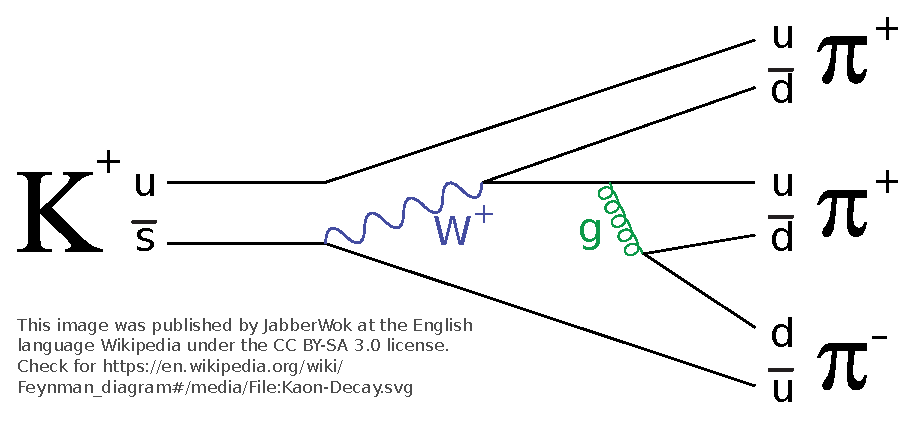
\includegraphics[scale=0.7]{./include/frontimage.eps}\\



    % examiners (Referenten)
    \vspace*{1.5cm}
    \Large
    \begin{center}
        \begin{tabular}[ht]{l c l}
        \iflanguage{english}{Supervisor}{Betreuer}: 
            & \hfill & \thesisreviewerone\\
        %\iflanguage{english}{Second Reviewer}{Korreferent}: 
        %    & \hfill & \thesisreviewertwo\\
        % uncomment if you want to provide info on your advisors
        %\iflanguage{english}{Advisor}{Betreuender Mitarbeiter}: 
        %    & \hfill & \thesisadvisorone\\
        %\iflanguage{english}{Second Advisor}{Zweiter betreuender Mitarbeiter}: 
        %    & \hfill & \thesisadvisortwo\\
        \end{tabular}
    \end{center}



    % working time
    \vspace{1cm}
    \begin{center}
        \large{{Bearbeitungszeit}: \thesistimestart \hspace*{0.25cm} -- %
                                   \hspace*{0.25cm} \thesistimeend}
    \end{center}



    % lowest text blocks concerning the KIT
    \begin{textblock}{10}[0,0](4,16.8)
        \tiny{KIT -- Universität des Landes Baden-Württemberg und nationales %
              Forschungszentrum in der Helmholtz-Gemeinschaft}
    \end{textblock}
    \begin{textblock}{10}[0,0](14,16.75)
        \large{\textbf{www.kit.edu}}
    \end{textblock}
\end{titlepage}

    
\chapter*{Erklärung zur Selbstständigkeit}
Ich versichere, dass ich diese Arbeit selbstständig verfasst habe und keine %
anderen als die angegebenen Quellen und Hilfsmittel benutzt habe, die %
wörtlich oder inhaltlich übernommenen Stellen als solche kenntlich gemacht und %
die Satzung des KIT zur Sicherung guter wissenschaftlicher Praxis in der %
gültigen Fassung vom 17.05.2010 beachtet habe.\\

\vspace{1cm}

\renewcommand{\arraystretch}{0} % for spacing in the tabular environment

\begin{flushright}
	\begin{tabular}{rr}
		Karlsruhe, den \thesistimehandin, & \hspace*{5cm}\\[0mm]
		\cline{2-2}\\[2mm]    % the last line has height 2mm due
		& \thesisauthor       % to \arraystretch=0
	\end{tabular}
\end{flushright}

\vfill

\begin{flushright}
	Als Ansichtsexemplar genehmigt von\\
	\vspace{1cm}
	\begin{tabular}{rr}
		Karlsruhe, den \thesistimehandin, & \hspace*{5cm}\\[0mm]
		\cline{2-2}\\[2mm]    % the last line has height 2mm due
		& \thesisreviewerone  % to \arraystretch=0
	\end{tabular}
\end{flushright}

\renewcommand{\arraystretch}{1}

\cleardoublepage


    \begingroup \let\clearpage\relax    % in order to avoid listoffigures and
    \tableofcontents                    % listoftables on new pages
    \listoffigures
    \listoftables
    \endgroup
    \cleardoublepage
    
    % Contents
    \MainMatter

    \chapter{Introduction}
    \section{The premise}

This document aims to create an entry point to unreal engine VR development. Hereby the focus is not necessarily on creating a full blown game mechanic, but rather on projects, which would be both achievable and beneficial in a scientific context.\\
Although this document aims to create sort of a general overview, it is being written specifically for the \textit{Institute of data processing}(IPE) at the KIT. The IPE has already conducted multiple VR projects. I will use them as an example to explain, what purpose a VR project could have in the scientific context:

\begin{itemize}
\item One project used the CAD models for the \textit{KATRIN} [CITATION] experiment and imported those as models into a VR setting, which can be used present the experiment to a broader public, which is not able to visit the restricted area for example.
\item Part of the research at the KIT campus north is the recording of x ray tomographies. Using this method researchers were able to create detailed 3D models of insects within fossils. There has been an effort to import these insect models into a VR setting. The capabilities of the unreal engine could help to animate the movement and behaviour of these long extinct species for example. An audience would be able to experience these animals first hand.
\end{itemize}

\section{document overview}

This document aims to achieve several things:

\begin{description}
\item[entry point] This document should provide a basic overview of the first steps to be taken, when starting VR development with the unreal engine, such as the installation of required programs and the setup of the needed hardware.
\item[choices] The success of a VR project is significantly determined, by the planning process or the general "vision" for the final project. There are some game-specific and also VR-specific design choices, that have to be well thought about when determining the initial goal of the project.
\item[tutorial] I will attempt to provide tutorial-like sections for chosen topics, which will be helpful for developing a first application scaffold.
\item[literature] The unreal engine is too big of a topic to be explained well in a single document. Thus, this document will not provide a "real" tutorial. Instead I will reference some literature and other resources, that have done a good job of explaining certain aspects of the topic.
\end{description}


    
    \chapter{First steps}
    % So this is supposed to be the section, where I explain how TCP and ethernet frames work
\section{Computer Networking}

\subsection{Reference models}

Communication between computer systems is achieved through the exchange of messages. For computers specifically these messages will be represented as a series of bits. But receiving an arbitrary series of bits from another maschine cannot be called communication. For a successful transmission of information, the receiving end needs to be able to make sense of these bits.\\
Transmitter and Receiver define a common protocol, which essentially defines what kind of information is sent at what position within the message.\\
Due to the complexity of computer networks, the communication within these is divided into multiple layers within a so called reference model. Each layer attempts to deal with a specific aspect of the communication process. These layers build upon the interfaces of the layers below them, create a new level of abstraction to then provide a higher-level interface to be used by those layers above them.\\
There are multiple reference models, but among the most popular ones is the hybrid reference model, which differentiates between 5 layers:\cite{ComputerNetworks}
\setlength{\fboxsep}{10pt}%
\setlength{\fboxrule}{0pt}%
\begin{figure}[h]
\centering
\fbox{\includegraphics[width=0.8\textwidth]{./img/hybrid_reference_model.png}}
\caption[The hybrid reference model]{The hyprid reference model}
\end{figure}

\begin{description}
\item[physical layer] As the lowest layer, it is responsible for the transmission of the individual bits. Since physical media are not discrete, it is the job of the transport layer protocols to define the modulations of the one and zero state into physical signals, which are being sent over the channel. On the receiving end those signals are being transformed back into a stream of bits. Examples for such modulations would be the usage of different voltages in cables or electro-magnetic waves of different frequencies to represent the binary states.
\item[data link layer] If errors occur during the transmission of the bit sequences, it is the data link layer's responsibility to detect and optionally correct these errors. Within the sender the data link layer packs the messages into \textit{frames}. On the receiving end, the protocol recognizes these frames within the bit stream of the physical layer. The delivery of those frames to the correct recipient requires the physical addresses of the target devices, the MAC addresses.\\
The frames of the data link layer can only be exchanged between directly physically connected machines.
\item[network layer] Most of the desired communication within computer networks goes beyond just physically connected machines. This wider scope of connected machines forms a logical network.\\
It is the network layer's task to forward packets within these logical network, over the borders of individual physical network segments.\\
For this a logical address (IP address) is defined.
\item[transport layer] The network layer ensures, that messages are routed from the sender to the correct receiver within a logical network. The transport layer enables communication of two individual processes or programs on those machines.\\
In this layer the running processes are identified by port numbers. So a process sending data to another process on another machine would have to supply the logical address of the target machine and the port number to which the target process is bound on that machine.
\item[application layer] The application layer is formed by all protocols, that interact directly with the application programs.\\
An example would be the HTTP protocol, which is used to view websites within a web browser. 
\end{description}

\subsection{Ethernet frames}
\label{sec:eth}

It is the protocols of the data link layer, that make sense of the bit stream of the physical layer. For this purpose, they define \textit{frames}. These frames define special bit sequences for the beginning and the end of a frame. Consequently machines listening on the network can recognize and identify individual frames. The frames make up logical units, which contain the addresses of sender and recipient, actual message data and additional error correction code.\par 

Ethernet frames are a protocol of the data link layer within the hybrid reference model. As the name suggests, it is used when transmitting messages in ethernet networks.\\
The protocol roughly consists of the following parts: A \textit{preamble}, which consists of 7 bytes. It is used to signify the start of a new frame. Next up it consist of the MAC address of the message destination and the message source, which make up 12 byte in total. Then there are 2 bytes for the \textit{type}. These two bytes are characteristic for a protocol of the upper layers, which use this frame to transport their messages. Every protocol is identified by their own byte sequence. The actual transmitted data is called the \textit{payload}. The payload can make up to 1500 bytes. Also, there are 4 bytes of \textit{CRC checksum}, which is used for error detection.\\
After the transmission of a frame there will be 12 bytes worth of \textit{interframe spacing}. These bytes are left empty to avoid interframe interference.\cite{ComputerNetworks}

\setlength{\fboxsep}{0pt}%
\setlength{\fboxrule}{0pt}%
\begin{figure}[h]
\centering
\fbox{\includegraphics[width=\textwidth]{./img/ethernet_frame.png}}
\caption[Architecture of an ethernet frame]{Architecture of an ethernet frame (simplified)}
\end{figure}

\subsection{TCP}
\label{sec:tcp}

The data link layer layers provides the possibility to transmit data from one physical machine to another. The network layer extends the "range" of transmission from physical networks to logical ones. By using the logical IP addresses and global routing infrastructure, data packets can be sent around the globe.\\
For some applications this might already be enough. But for many it also is not.\par 

The \textit{transmission control protocol (TCP)} is a protocol of the transport layer within the hybrid reference model. It builds upon the possibilities of the network layer. It extends the network layer with a much desired reliabality: It is guaranteed, that data segments reach their destination fully intact and in the correct order. The sender also automatically sends lost or unacknowledged TCP segments again.\\
From a top level perspective TCP connections can be opened and closed much like a file. Data that is being pushed into the connection is treated as an ordered data stream. This stream of data is potentially very long. Most likely longer than the maximum payload size of the data link layer. Thus the data is split into segments, which will be sent individually.\\
As part of the protocol, TCP appends its own header data in front of the segment data. The TCP header is in total 20 bytes long and consists of the following core information: The IP address of the sender and the receiver, a protocol ID, the length of the segment, the port number of the application on sender and receiver side, the sequence number, the acknowledge number a checksum and the flags for SYN, ACK and FIN.
\cite{ComputerNetworks}

\setlength{\fboxsep}{2pt}%
\setlength{\fboxrule}{0pt}%
\begin{figure}[h]
\centering
\fbox{\includegraphics[width=0.8\textwidth]{./img/tcp_header.png}}
\caption[Structure of a TCP header]{Structure of a TCP header. Important parts highlighted in green}
\end{figure}

% here I sort of go into the dynamic functioning of the TCP protocol
% Here I just sort of introduce the concepts, but dont flesh them out yet.
The sequence number, abbreviated as "seq" and the acknowledgment number, abbreviated as "ack" are most important to the direct function of the TCP protocol.\\
The seq number represents the index of the current packets first payload byte within the broader scope of the complete data stream. The ack number signifies what data has been received by the other side. It will be set to the index within the global scope of the communication, which will be expected next.\par 

When establishing a connection the client sends a TCP packet to the server. For this package the \textit{SYN (synchronize)} flag is set. Additionally the seq number of this packet is set to the beginning of the global data stream, which we assume to be zero \footnote{We only \textit{assume} it to be zero here for simplicity. In reality the protocol uses a randomly determined starting number}, since this is were the transmission of global data starts. We will call the seq number for data from the client to the server "$x$".\\
The server replies with a packet, which has both the SYN and the \textit{ACK (acknowledgement)} flag set. The ACK flag signifies to the client, that the server is willing to initiate a communication channel. The ack number of this reply packet will be set to $x+1$. It points to the index of the next expected data batch. We will also assume, that the seq number for this packet will be set to zero, to indicate the start of the data stream from server to client. This second sequence number will be called "$y$".\\
The client yet again replies with a packet, which has only the ACK flag set, implying that the synchronization has been finished and the established connection is also confirmed by the client. This third package now has the sequence number $x+1$, which is expected by the server. It also declares $y+1$ as its ack number, as that is the next expected index within the server-to-client data stream.\\
This process of establishing a TCP connection is also known as the \textit{three way handshake}.\par

\setlength{\fboxsep}{2pt}%
\setlength{\fboxrule}{0pt}%
\begin{figure}[h]
\centering
\fbox{\includegraphics[width=0.9\textwidth]{./img/tcp_connection.png}}
\caption[Structure of a TCP connection]{Basic initialization process of a TCP connection with the three way handshake and data transmission process}
\end{figure}

As it became obvious, data can be transmitted from the client to the server as well as vice versa. The seq number denotes the current index of the two directional data streams. The ack number is a representation of either sides expectation of which seq number they have to expect within the next received packet.\\
Keeping a record of the actual position within the data stream as well as the expectation of the next data enables the detection of data loss: The ack number acts as a confirmation of what has actually been received on the other end of the channel. does the ack number of the server reply for example not match the seq number of the next client packet, it is likely, that the previous packet never made it to the server.  In such a case the TCP protocol will send the lost package again and resume afterwards, without bothering the application layers perceived functionality of the TCP channel.\\
Additionally the sequence numbers will guarantee, that data segments are received in the correct order, as well as duplicates being recognized\footnote{Packets being lost, duplicated or received out of order happens quite often on a network layer level. This is due to the complex routing infrastructure involved in sending packets over multiple  physical networks}.\cite{ComputerNetworks}

\section{SIMD Instruction Sets}
\label{sec:simd}

Many modern processor architectures support so called \textit{single-insturction multiple-data (SIMD) Instructions sets}. A SIMD-capable processor includes computational ressources that leverage concurrent calculations using multiple data values. These inherently concurrent instructions have a major performance advantage compared with traditional instructions.\cite{ModernAssembly}\\
Many modern "high-level" programming languages are not yet able to utilize SIMD instructions properly. This can be due to the very specific instructions being hard to implement into high level concepts such as object orientation. Another reason might be to maintain a general device support. New instruction sets are being introduced continually. These additional instructions are very architecture specific and are only supported by specific processor models. On older machines a newer standard of these instructions will not be supported, breaking backwards compatibility for some applications.\par 

For the C programming language there is a concept called \textit{intrinsics}. Usually functions are stored in libraries, but some functions are built into the compiler itself. These functions are called \textit{intrinsic} functions. For such a function the code, which describes this function is usually inserted inline by the compiler, thus removing the overhead of an actual function call. Additionally, the compiler often has knowledge of the inner working of these functions. This enables the compilers optimizer to make inline functions to perform even better than inline assembly code.\cite{CompilerIntrinsics}\\
With the C language many of these SIMD instructions are being implemented as intrinsic functions. This enables to take full advantage of the improved performance these new instructions provide. A full reference of these intrinsics, their parameters and usage can be found in \cite{IntelIntrinsicsGuide}

\section{X-Ray Tomography}

% Also hier sollte ich ein bisschen einen Überblick über die theoretischen Grundlagen
% geben, weshalb ich das alles hier überhaupt mache. Also erklären inwiefern man 
% durch x ray tomography überhaupt einen Aufschluss über die interne Strukur eines 
% Objektes bekommt

% Aber um erhrlich zu sein ist der Teil nicht allzu wichtig

lul

\section{The Phantom Camera model v2640}

% Ein Bild von der phantom camera. Nur damit der Leser sich mal ein Bild davon machen 
% kann wie solche high speed cameras denn aussehen.
\begin{figure}[h]
	\caption[Phantom models v1840 and v2640]{The phantom camera models v1840 and v2640 \footnotemark}
	\includegraphics[width=\linewidth]{../img/phantom_image.png} 
	\label{fig:phantom1}
\end{figure}
\footnotetext{image source: \url{https://www.phantomhighspeed.com/-/media/project/ameteksxa/visionresearch/images/product/uhs/v18n26combo.png}(accessed 2019-07-18)}

% Hier sollte ich die Specs der Kamera aufzählen
The Phantom Camera v2640 is one of the newest additions to the ultra-high-speed imaging family of Vision Research. Its core features are \cite{PhantomDatasheet}:
\begin{itemize}
\item A 4Mpx sensor, enabling frames with a maximum resolution of 2048 x 1952 at a bit depth of 12 bit.

\item Various available modes, which include standard, high-speed and binned frame acquisition. The high-speed-binned mode features a maximum frame rate of 25030 FPS at a resolution of 1024 x 976 pixels 

\item Up to 288GB of internal RAM memory, which can be partitioned into up to 63 cines\footnote{A \textit{Cine} is a custom storage data format for a recording of multiple cines developed by Vision Research. It is used internally in phantom cameras to organize multiple recordings without overriding previous ones.}. The record duration is even more extendable through the use of the Phantom CineMag \texttrademark (1TB and 2TB available) \footnote{The CineMag is an additional storage device, which can be inserted into the camera to extend the internal memory}

\item A low noise of 7.2 e- and a high dynamic range of 64dB

\item Multiple I/O Ports. Among those are 4 Programmable I/O ports. Possible configurations include the usage of an external trigger source, a memory gate function \footnote{The \textit{memgate} function will block the saving of frames into the internal as long as the supplied pulse is LOW/HIGH (configurable). This enables to time the acquisition of frames exactly with the duration of the process to be observed}, frame sync signal and more. The camera also contains 1GB and 10GB ethernet ports for control signals and data transmission. The 10GB ethernet connection can transmit up to 600MB/s of image data, \textit{on optimized systems}.
\end{itemize}

\section{The LibUCA Framework}

The Unified Camera Abstraction Library, or LibUCA in short, is one building block of the UFO framework. The UFO framework was developed to provide "A Scalable Platform for High Speed Synchrotron Imaging". The platform features the handling of the full imaging process from the actual recording to processing and long term data storage.\cite{UFOPaper}\par
LibUCA in particular exposes a light-weight API interface to the UFO core, which enables to abstract common camera operations such as recording triggering and reading out the internal memory. This abstraction allows almost any camera to be integrated into the UFO-workflow, as long as an additional UCA-plugin is developed.  These plugins have to communicate with the camera and expose the result of this communication to the common entry points of the LibUCA library.\\

% Ein Bild welches die Architektur von libuca verdeutlicht
\begin{figure}[h]
	\caption[LibUCA architecture]{LibUCA architecture overview \footnotemark}
	\includegraphics[width=\linewidth]{../img/libuca_architecture.png} 
	\label{fig:phantom1}
\end{figure}
\footnotetext{image source: \url{https://libuca.readthedocs.io/en/latest/_images/architecture.png}(accessed 2019-07-18)}

LibUCA itself is implemented in the C programming language and the Glib\footnote{\textit{Glib} is a C library, which aims to provide advanced programming concepts to the relatively basic C programming language. Glib eases the use of object oriented programming, although not naturally supported by C. It also simplifies handling of strings, files, threads and more.} library.[CITATION GITHUB] As such plugins have to be developed as C as well. Through the use of the object oriented paradigms provided by GLib, this can be achieved by subclassing the basic \texttt{UcaCamera} class. For a minimal implementation of a plugin, the following virtual methods have to be overriden with custom code:\cite{LibucaDoc}

\begin{itemize}
\item \texttt{start\_recording}: This method has to make all necessary preparations so that every subsequent call to the \texttt{grab} method returns an image array.

\item \texttt{stop\_recording}: Stops the recording so that subsequent calls to the grab method fail.

\item \texttt{grab}: Has to return an image in the form of an array, where each pixel is represented by a 16 bit integer value.
\end{itemize}



    
    \chapter{Design Choices}
    
\section{The PH16 camera protocol}

% Ich denke in dem ersten Kapitel hier sollte ich zunächst mal ein bisschen beschreiben 
% wie man denn überhaupt mit der Phantom kommunizieren kann. Also wie man sich mit ihr 
% verbinden kann und and welche Ports und sowieso man etwas schicken kann
\subsection{Communication with the camera}
The phantom camera v2640 provides two ethernet ports to communicate with a computer. One port supports the 1GB ethernet standard, the other port supports the 10G standard. Control commands, as well as image data can be transmitted using both ports. The 10G port however additionally supports a fast data transmission using raw ethernet frames instead of a managed TCP conversation, effectively minimizing transmission overhead. Thus the 10G connection is to be prefered when aiming for the highest possible data throughput.\cite{PhantomDatasheet} \par
Each phantom camera comes shipped with a static IP address. This IP address is in the range 100.100.x.x for 1G connections and 172.16.x.x for the 10G port, where x is substituted with the product specific numerals. Consequently the the connected computer has to be configured to use the same IP range on the affected network card. It is recommended to assign the computer with the static IP 100.100.100.1 or 172.16.1.1 respectively.\cite{PhantomManual}\\
If everything is configured correctly, a connection to the camera can be established via telnet. Using the default telnet port with the username \textit{user} and password \textit{user} will open a remote access console to the unix based operating system of the camera. Alternatively a TCP connection can be established to the port 7115. This ports accepts control commands of the PH16 protocol. The PH16 protocol is a custom network protocol developed by Vision research and used to communicate with phantom cameras. All further sections about the PH16 protocol are based on the given  protocol specification:\cite{PH16Protocol}

% Ich denke ich sollte die cine structur vorher erkären bevor ich im nächsten 
% Abschnitt in so gut wie jedem Satz das Wort "cine" erwähe und kein Leser eine 
% Ahnung davon hat was ich meine.
%\subsection{The cine structure}

% Ich denke ich sollte mich bei den Strukturen nur auf die wichtigsten beziehen, die 
% dann nachher auch relevant werden, damit die Liste nicht allzu lang wird.
\subsection{Controlling camera behaviour}
Configuring the behaviour of the camera is mainly done by setting according values to its internal properties. The internal unit structure is organized by having a set of top level structures, where each of them is separated into its own set of sub properties. The most relevant unit structures for the PH16 compliant camera models consist of the following:

\begin{description}
\item[info] General information about the camera configuration. This includes version numbers for hardware, firmware, sensor etc. for example as well as information about things like the resolution, maximum and minimum exposure time as well as frame rate.
\item[hw] (Abbreviation for "hardware") Factory-adjusted calibration settings
\item[c\#] The cine table. A cine is a special data format, developed by Vision Research, used to store recorded frames. Within the cameras internal memory a cine consists of a set of properties and the actual data storage. The properties describe the settings for the frame acquisition into this particular cine. The properties of a cine can be accessed through its indexed name. Each cine is named by the letter "c" followed by its index, such as "c1" for example. 
\item[defc] (Abbreviation for "default cine") This structure contains general setting about the nature of a recording. The properties defined here will be copied to each individual cine, when it is created. The settings for each cine can be modified individually afterwards.
\item[cam] Global settings for the camera, which aren't tied to a particular cine.
\item[eth] Global settings about the ethernet interface, including the IP and port which the camera is operating on.
\end{description}

% Hier will ich nur den basic syntax ein bisschen anreißen. Also der Aufbau command 
% und parameters und dann, was die camera darauf antwortet
\subsection{Control commands}
Active communication with the camera is performed by sending control commands in the form of strings to the TCP port 7115. The syntax of these strings consists of the command keyword, optionally followed by command parameters and terminated by the newline character "\textbackslash r\textbackslash n":
% Shows the basic syntax composition for a control command
\begin{lstlisting}
"<command_name> <parameters> \r\n"
\end{lstlisting}

For every command the camera will send a response. If the command is purely of declarative nature, the camera will send the string "OK!". If, on the other hand, the command requests data from the camera a string containing this data will be sent as the response.\\
In case the sent command is formed incorrectly or the described action is not applicable by the camera, it will send an error message instead. This error message is of the following format:
\begin{lstlisting}
"ERR: <explanatory_string>"
\end{lstlisting}

% Das sind denke ich die wichtigsten und einfachsten Kommandos. Also get und set
% sollten auf jeden Fall mit dabei sein.
\subsection{Getting and setting camera properties} \label{sec:phgetset}
The most simple commands to interact with the camera are the \texttt{get} and \texttt{set} operations. These commands are used to manipulate the properties of camera to change it's behaviour in the future.\par
The \texttt{get} command reads out the value of one or more properties. The command syntax consists of the keyword followed by the name of the property to be read. This property name could either be a specific property specified as "<top level structure>.<property>":
\begin{lstlisting}
get <property_name>
\\ Example (exposure time)
get defc.exp
\end{lstlisting}
The \texttt{set} command assigns a new value to one of the properties. It is important to keep in mind, that all properties can be read, but not all of them have write access. The set command can only be used on those properties that have been explicitly marked as r/w in the protocol specification. Trying to do otherwise will result in an error.\\
The syntax consists of the keyword followed by the name of the property, specified in the same way as with the get command, and the new value to be assigned: 
\begin{lstlisting}
set <property_name> <value>
\\ Example (exposure time)
set defc.exp 100000
\end{lstlisting}

% Hier will ich erklären wie der Aufnahme Prozess funktioniert und weil das thematisch 
% ganz gut zusammenpasst kann ich hier auch noch den trigger mit rein packen
\subsection{Making a recording}
To record an event with the camera, the first step is to set the camera into the recording state. This is achieved by using the \texttt{rec} command. The syntax is just the rec keyword followed by the cine number:
\begin{lstlisting}
rec <cine_number>
// Example (recording into cine with index 1)
rec 1
\end{lstlisting}
The cine number is the index of the cine partition of the internal memory into which the frames are supposed to be saved. After the \texttt{rec} command has been issued, the camera will start to capture frames and save them into the specified cine. For the capture process it will use the parameters, that are specified by the parameters of the "c1" property structure. This includes parameters such as exposure time, frame rate etc.\\
The camera will continue to fill the internal memory until one of two things happens: 
\begin{itemize}
\item The cine memory partition does not have any more space for additional frames.
\item A trigger event occurs within the camera. This trigger event can either originate from an actual electrical pulse to the trigger port of the camera or it could be a software trigger command.
\end{itemize}

A software trigger will be initiated by the \texttt{trig} command. The syntax of the command is just the trig keyword without any parameters. Once the trig command has been received by the camera it will simply simulate a hardware trigger.\\
Once a trigger has occurred within the camera it will only record as many frames as previously specified in the \textit{post trigger frames} property (defc.ptframes). After this amount of frames, the camera will exit the recording state and wait for a new \texttt{rec} command.

% Hier erkläre ich dann wie man Bilder ausliest also sowohl für 1G also auch für 10G
% Das ist denke ich der wichtigste Teil des ganzen Kapitels, weil es den 
% Grundstein legt für die spätere Erklärung, wie ich den Auslese Algorithmus gemacht 
% habe.
\subsection{Readout of image data} \label{sec:phreadout}
After a recording has been made, the image data still has to be transferred from the internal memory of the camera to the computer for further processing. For this the camera provides two different commands:
\begin{description}
\item[img] The img command is the default way of transferring image data. It uses TCP sockets and is available both on the 1GB and the 10GB port. Due to the overhead of TCP communication this process is rather slow.
\item[ximg] The ximg command can only be used on the 10G ethernet connection and is specifically designed for fast transfer. It uses raw ethernet frames to minimize overhead.
\end{description}

\paragraph{The IMG command}
Using the \texttt{img} command, image data is not being sent over the control connection. The TCP connection established over port 7115 will always be reserved for just control commands. This means a secondary channel has to be opened for the data to be transmitted.\\
The control connection is established by the computer. The computer has the role of a client and the camera the role of a server. All interactions are initiated by the computer: A request is being sent, to which the camera sends a response. For the data connection on the other hand, the camera is the main actor, which sends the data stream. Thus for the data connection the computer has to act as a server, which responds to the incoming data, while the camera initiates the transmission.\\
To start such a secondary data connection, the \texttt{startdata} command has to be sent over the control connection first. The startdata command expects a port number as a parameter:
\begin{lstlisting}
startdata {port:<port_number>}
// Example (start data connection on port 8999)
startdata {port:8999}
\end{lstlisting}
After receiving this command the camera will attempt to open a TCP client socket to connect to the computer at the given port. For this a TCP server socket has to be running on the computer already, or else the command will result in an error. Only after this connection has been properly set up, subsequent \texttt{img} commands can succeed.\par
The \texttt{img} command syntax expects the following parameters:
\begin{description}
\item[cine] The index of the cine from which to read the image. The value -1 is the special case of returning live images. This will work even if the camera has not recorded anything yet and the image will, whatever the camera "saw" in the moment, when the command got executed.
\item[start] An integer number for the index of the frame \textit{within the chosen cine}, which is to be the first transmitted cine
\item[cnt] An integer number of how many frames after the \textbf{start} frame are supposed to be transmitted.
\item[fmt] A string identifier for the format in which the frames are supposed to be encoded for the transmission. The PH16 protocol offers a few different options where a single pixel is being encoded with 8, 10, 12 or 16 bit.  
\end{description}
\begin{lstlisting}
img {cine:<cine_index>,start:<start_index>,
	cnt:<frame_amount>,fmt:<format>}
// Example (single live frame, 12 bit encoding )
img {cine:-1,start:0,cnt:1,fmt:P12L}
\end{lstlisting}
Right after the img command has been received, the camera will start to send a byte stream over the data connection socket. The data does not contain any overhead. The first byte transmitted belongs to the first pixel of the first frame.\\
As for the reconstruction on the computer side: The value for each pixel can be determined by reversing the encoding specified by "fmt". The list of the pixels can then be aligned into a 2 dimensional image matrix by using the resolution of the camera.

\paragraph{The XIMG command}
The \textit{ximg} command does not need an additional setting up step. The command expects the same parameters as the \textit{img} command, with the additional destination (dest) parameter:
\begin{lstlisting}
img {cine:<cine_index>,start:<start_index>,
	cnt:<frame_amount>,fmt:<format>,dest:<destintation_mac>}
// Example (single live frame, 12 bit encoding )
img {cine:-1,start:0,cnt:1,fmt:P12L,dest:2fde67h6}
\end{lstlisting}
The destination parameter is supposed to contain the MAC address of the network card of the computer, which is used to maintain the 10G connection with the camera.\\
Additionally the \texttt{ximg} command only supports a limited subset of transfer formats for the "fmt" parameter.\\
After receiving the command, the image data of the specified images is simply to the ethernet connection as raw ethernet frames. Aside from the ethernet header, they will only contain the image bytes. This of course makes it necessary to have program running on the computer, which reads all the ethernet frames on the connection.
[OPTIONAL: AN IMAGE OF HOW THE ETHERNET FRAME IS LAYED OUT]

% Also mir ist aufgefallen, dass ich das discovery protocol auch noch erklären sollte, 
% weil ich darauf bei dem architecture overview für die Mock einegehen will, wie viele 
% Threads da gleichzeitig laufen müssen.
\subsection{The discovery protocol}
The PH16 protocol also supports a "discovery protocol". With the use of the discovery protocol the IP address of a specific camera model does not have to be know in advance. A computer can simply send a UDP broadcast message containing the string \texttt{"phantom?"}. If this UDP package has been sent to the network, to which a camera is also connected to, it will respond upon receiving it. The IP of the camera will then be know through the meta data of the UDP response package.

% %%%%%%%%%%%%%%%%%%%%%%%%%%%%%%
% HIER FÄNGT DIE NEUE SECTION AN
% Nachdem ich ja jetzt im letzten Kapitel einen Überblick über das Protokoll selber 
% gegeben habe, sollte ich in diesem Teil PhantomCLI beschreiben. Ich denke was auf 
% jeden Fall rein sollte ist: 1) Wie man es benutzt, 2) Wie die Mock aufgebaut ist. 
% 3) Wie das main interface aufgebaut ist.
\section{PhantomCLI - camera command line interface}
% Hier sollte so eine Art Einleitung hin, also eine Erklärung, was ich mir gedacht 
% habe und was mein Ziel damit war.
Before working on the actual plugin, I wanted to get a better understanding of how the camera and the PH16 protocol worked. So I developed some command line utilities for testing and handy common operations.\\
my initial goals were to implement at least a getting and setting of properties, the starting of recordings and the readout of images.\\
Furthermore I wanted to build a simple \textit{mock} program of the camera. This was due to the fact, that I only had limited access to the actual camera and I did not wanted to limit all the testing of my code to these limited time frames. A simple simulation of the network behaviour of the camera would be enough for most situations.

% Ich lasse diese Sektion erstmal aus, weil ich mir gerade nicht mal sicher bin, ob ich 
% die überhaupt brauche. Weil ich meine ganz ehrlich, wer kennt Python nicht?
\subsection{Used technologies} \label{sec:phantomcli_used_tech}

\paragraph{Python}
The \textit{PhantomCLI} project is written in the Python[CITATION] programming language. Python is a high-level programming language. It supports various programming paradigms such as imperative, functional and object oriented programming. It is an interpreted language, which makes it widely platform independent. Python is a general purpose programming language, with a big standard library and a rich ecosystem of third party libraries. Such libraries include various networking and command line frameworks, which will be needed by this project. Together with it's simple syntax, python offers a good foundation for rapid development.

% Ich denke es macht durchaus Sinn einmal kurz zu erklären, wie PyPi funktioniert, 
% damit man dann später in der section über das tatsächliche CLI einfach sagen kann
% "installieren kann man es mit pip."
\paragraph{PyPi - Python Package Index}
PhantomCLI is being distributed, using the PyPi repository. The \textit{Python Packaging Index}[CITATION] is a software repository for the Python programming language. It has become the standard choice for distributing python libraries as well as applications. Once a program has been uploaded to PyPi it can be easily installed from the terminal, using the package management program \textit{pip}. For an installation with pip, only the name of a package has to be known:

\begin{lstlisting}
$ pip install package_name
\end{lstlisting}

All additional dependencies of any installed package will be automatically resolved. PyPi also supports semantic versioning and will keep all previously uploaded versions.

\paragraph{Click}
For its command line interface, PhantomCLI uses the \textit{Command Line Interface Creation Kit (click)}[CITATION] framework. Above all other Python CLI libraries click features a simple API by using the Python decorator syntax, while sill maintaining powerful customisation options.

% Hier will ich beschreiben, wie die API des Programms ausssieht. Also wenn man
% phantomcli jetzt zum Beispiel benutzen wollen würde als library, wie man dann von 
% "außen" über die API mit der Kamera kommuniziert.
\subsection{The socket API}
The API\footnote{\textit{Application Programming Interface}. An API usually describes a simple set of actions or objects, exposed by a library. These exposed functions can be used to build an application on top of the library, while abstracting the underlying complexity.} of the \textit{PhantomCLI} library consists of a single class. The \texttt{PhantomSocket} class (figure \ref{fig:uml1}) can be instantiated to create a \texttt{PhantomSocket} object.
% Das UML Diagramm für PhantomSocket
\begin{figure}[h]
	\caption[PhantomSocket UML]{UML Diagram for the PhantomSocket class}
	\includegraphics[width=\linewidth]{../img/PhantomSocketUML.png} 
	\label{fig:uml1}
\end{figure}
% Hier erkläre ich die Parameter für den Konstruktor
% In der Auflistung fehlen noch ein paar parameter, aber ich weiß auch ganz ehrlich nicht 
% ob man die noch unbedingt braucht...
To create new \texttt{PhantomSocket} object the following parameters can be passed to the constructor:
\begin{description}
\item[ip] The required argument for the creation of a socket class is a string, which contains the IP address of the specific phantom camera to connect to.
\item[timeout] The timeout specifies an integer time in seconds. After this time has passed and the TCP socket has not yet received a response to a previous request, the program will raise an exception. The default is 10 seconds.
\item[data\_ip] A string containing the IP of the computer running the PhantomCLI program. This will be the IP, onto which the data server will be bound to while receiving image data. Default is localhost
\item[data\_port] An integer port number. The data server, which will receive the image data, is going to be operating on this port. Thus this will have to be an otherwise unused port. Default is 7116
\item[img\_format] A string containing the name of the format to be used to transmit the image data from the phantom to the computer. Default is \textit{P16}
\item[network\_type] A string, which specifies the type of ethernet connection, which is used to connect to the phantom. The string "e" refers to a 1GB ethernet connection, while "x" is the 10GB connection.
\end{description}
% Hier erkläre ich was die einzelnen Methoden machen
The \texttt{PhantomSocket} class provides the following public methods to interact with the phantom camera:
\begin{description}
\item[connect] After creating the object, it is not yet connected to the actual camera. By calling this method a new TCP socket will be created and connected to the camera.
\item[disconnect] Closes the connection to the camera and deletes the network socket object.
\item[get] Given the name of an internal structure, this method sends a \texttt{get} command to the camera and returns the response string.
\item[set] Assigns a new value to one of the internal attributes of the camera
\item[startdata] Creates a new threaded TCP Server object. Then it sends the \texttt{startdata} command to the phantom, so the camera can create a new data connection.
\item[img] Sends the "img" command to the camera. The camera will then start to transmit the image data over the secondary data connection. This method blocks until the data server classifies the transmission as completed. Creates and returns a PhantomImage object from the data in the data server.
\item[ping] Sends a ICMP ping to the IP address of the camera. Returns True, if the camera replied and False otherwise
\item[discover] This static method will send a UDP broadcast message into the network. Returns a list of dictionary structures, where each dictionary contains the informations about a cameras name and IP address.
\end{description}

% Hier will ich reinschreiben, wie die Mock funktioniert.
% Was das angeht denke ich, ich werde nicht undbedingt genau die Klassen beschreiben, 
% sondern werde nur so obeerflächlich beschreiben, welche Threads alle gleichzeitig 
% laufen müssen und wie der flow eines Handlings ist.
% Am Ende vielleicht noch ein bisschen darauf eingehen, was noch nicht so 
% funktioniert wie ich das haben will, bzw. wie es sein sollte.
\subsection{The phantom Mock}
The \texttt{PhantomCLI} project also provides a mock class \texttt{PhantomMockServer}. This mock server runs as a thread, so that once it is started, it's functionality will not block the program execution.\par 

\paragraph{the thread structure}
% Hier will ich erklären, wie die threaded server funktionieren. Also generell die Meta 
% Struktur der Mock. welche Threads alle auf einmal laufen.
The \texttt{PhantomMockServer} class inherits from the \texttt{ThreadedTCPServer} class of pythons standard library module \textit{socketserver}[CITATION]. Server classes from the socketserver module generally work by providing a method \texttt{serve\_forever}. Calling this method will be blocking the program execution, by making the internal socket continously listening for incoming connections. Once a connection has been established the server will create a new "Handler" class. The socket connection is then passed to this handler instance, while the server itself will continue listening for new incoming connections. The actual protocol specification has to be implemented within the handler class. The \textit{threaded} version of the Server class will run each newly created handler as a thread, so that the listening process is not interrupted.\par 
Since the \texttt{server\_forever} method is blocking even for the threaded version of the server class, the \texttt{PhantomMockServer} creates an additional thread. This additional thread will run the \texttt{server\_forever} method. Thus calling the \texttt{start} method on the \texttt{PhantomMockServer} will not be blocking, as the listening loop is executed in a thread, as well as all future connections handlers.\par
Additionally to the main socket handling, the \texttt{PhantomMockServer} starts and maintains two additional threads. The first one being an instance of the \texttt{PhantomDiscoveryServer}. This class inherits from the base class \texttt{ThreadedUDPServer} from the python module \textit{socketserver}. It creates a listening socket for incoming UDP packages. The corresponding handler class implements the phantom discovery protocol.\\ The second thread is an instance of the \texttt{PhantomCamera} class. This class simulates the actual camera behaviour. It contains the properties with which camera behaviour can be controlled. These properties can be read and modified. Additionally the camera object can simulate the start of a recording, a software trigger and the generation of frames. 

[HIER MUSS NOCH EIN BILD REIN; WAS DAS ÜBERSICHTLICHER MACHT]

\paragraph{command handling}
% Hier könnte ich erklären wie die einzelnen commands dann tatsächlich gehandled werden
Once the \texttt{PhantomMockServer} receives an incoming socket connection, this open connection is being passed to a handler object for further processing. This handler instance contains the implementation of the command handling. This includes the decision about which command has been received, executing this command and generating a reply.\par 
At first the whole command string is being received and parsed. The parsing is being done by a parse tree, based on a custom grammer definition. The python package \textit{parsimonious}[CITATION] is being used for the definition of the PH16 protocol grammer.\\
After the parsing process the command name of the request is used to call the specific handling method for that command. The parsed command parameters are passed as arguments to this method. Currently the following PH16 commands are supported by the mock:
\begin{description}
\item[get] Retrieves the value to the given property name from the simulated \texttt{PhantomCamera} and sends it as a response
\item[set] Sets the new value to the property of the simulated \texttt{PhantomCamera}
\item[startdata] Attempts to create a new TCP client connection at the given port.
\item[img] Generates a new image from the \texttt{PhantomCamera} instance. Sends the raw image data through the data client.
\item[ximg] Generates a new image from the \texttt{PhantomCamera} instance. Sends the raw image data as a ethernet frame to the network.
\item[rec] Starts a recording on the simulated \texttt{PhantomCamera}. This will cause the camera to start generating frames with the set frame rate, until a software trigger stops occurs. 
\item[trig] Issues a software trigger on the simulated \texttt{PhantomCamera}, which will 
stop the recording after the acquisition of the post trigger frames.
\end{description}
[HIER MUSS NOCH EIN BILD REIN; WAS DAS ÜBERSICHTLICHER MACHT]

\paragraph{Limits}
% In einem letzten paragraphen dann noch die momentanen limitations
In it's current state the mock of the phantom's behaviour supports the most basic functionality with the getting and setting of properties as well as the acquisition of frames. Working with this basic version will pose the following limits:\\
On the one hand the mock does not even support all the commands of the PH16 protocol. The protocol defines many more commands, which include creation of user profiles, the transmission of timestamp meta data and manipulation of network settings among many others.\\
On the other hand it does not accurately reflect camera behaviour. For example: The mock supports the start of a recording using the "rec" command, and a software trigger with "trig". This is a rather complex process in the actual camera. It includes the setting and changing of various properties and it affects various different cine partitions. The mock however currently only supports the acquisition of frames into a single, central list and the process does also not affect any properties.\\

% In diesem Kapitel mache ich ein bisschen Werbung, bzw. ich erkläre wie man phantom cli 
% einfach so von der Kommandozeile aus benutzt und verlinke auf meine Dokumentation
\subsection{The command line interface}

% Als erstes sollte hier eine Sektion hin, wie man das Programm installiert
Aside from the API, the \textit{PhantomCLI} project also features a command line interface. The command line interface was designed to provide quick access to various common operations while dealing with the phantom camera.\\
It can be installed by using \textit{pip}(sec.\ref{sec:phantomcli_used_tech}) to acquire the package "phantom-cli":

\begin{lstlisting}
$ pip install phantom-cli
\end{lstlisting}

The installation process will automatically create the bindings for the terminal commands, if pip is being executed with super used permissions.\par

% Hier sollte ich einfach aufzählen, wie man die Sachen benutzen kann
Currently, the following commands are supported by the \textit{PhantomCLI} package:

    
    \chapter{Ressources}
    \section{chapter overview}

in this section I will introduce some helpful resources in the form of books and websites, which will be helpful for the development of VR project with the unreal engine.

% Include a small summary of all the following sections, so that 
% a reader can quickly skim over, which ressource might be the 
% most interesting at the moment

\begin{description}
\item[Unreal for Mobile and Standalone VR] The focus of this book is specifically on development for mobile VR hardware, although all the topics described are also applicable for \textit{tethered VR platforms}\footnote{Tethered VR platforms are those platforms, which need mounted basestations to track the position of the user. These platforms have the advantage of offering a 6 DOF (degree of freedom) VR experience in contrast to the 3 DOF of mobile VR  platforms}.\\
This book includes general advice for the setup of a development pipeline, tools and design choices. Furthermore it includes two in depth tutorials: One for developing an interactive product showcase and another for developing a full game with all essential game mechanics.
\end{description}

\section{Book \textit{Unreal for Mobile and Standalone VR}}

This book can be acquired for free from the KIT library\cite{KitBib}, when accessed from the KIT wifi or a VPN, using the following URL:

\url{https://link.springer.com/book/10.1007%2F978-1-4842-4360-2}

\setlength{\fboxsep}{0pt}
\setlength{\fboxrule}{0pt}
\begin{figure}[h]
\centering
\fbox{\includegraphics[width=0.6\textwidth]{./fig/cover_unreal_mobile.png}}
\caption[Unreal for Mobile and Standalone VR]{cover of the book "Unreal for Mobile and Standalone VR"}
\label{fig:unrealmobilecover}
\end{figure}

\paragraph{Chapter 3: Before you start}

The third chapter from the book was the basis for the chapter \ref{chap:designchoices} about design choices in this document. Everything mentioned and a lot more is described here in detail.\\
Furthermore the third chapter includes some nice tips on \textit{low hanging fruits}\footnote{the term describes aspects of a project, which can improve the project a lot and are easy to achieve} of every VR project. 

\paragraph{Chapter 4: Unreal for VR}

The main focus of this chapter is on creating a VR project for the \textit{Oculus Go} platform specifically. The basic tutorial for setting up simple motion controller locomotion blueprints is generally applicable nonetheless.

\paragraph{chapter 6: Creating an Interactive VR Presentation}

This chapter is a full on tutorial on how to create a VR product presentation. Since a product presentation has a lot in common with a presentation for a science project, this chapter is the most relevant to get started with a project.\\
The chapter roughly contains the following content:
\begin{itemize}
\item Pipeline for creating the scene aesthetics using Unreal and Blender
\item lighting the scene
\item basic environment interactions with floating UI buttons and sequencer animations
\end{itemize}


    
	\chapter{Tutorials}
	\section{Experiments at TOPO-TOMO}
\subsection{Experimental setup}
\subsection{Previous accomplishments}

\section{Testing the camera}
\subsection{speed}

	
    %\emptychapter[3]{ROOT Routines}     % usage: \emptychapter[page displayed 
                                        %        in toc]{name of the chapter}
    %\chapter{Conclusions}
    %\section{Summary}

% What do I even want to say about it?
% - Programming the cli was a very good, way to get to know the 
% camera protocol, especially programming the mock, where I tried 
% to reverse engineer the cameras inner workings
% - The mock really helped the development process, as some of the 
% testing did not have to be done with the camera fully set up.
% - A quick out of the box tool to test the most common operations 
% with the camera, which does neither rely on using the telnet 
% connection and memorizing the protocol or compiling the whole 
% libuca pipeling
\subsection{PhantomCLI command line tools}

The PhantomCLI\footnote{Available at \url{https://github.com/the16thpythonist/phantom-cli}} package provides simple command line tools to perform basic interactions with the phantom camera. Furthermore a simple camera mock simulation was implemented, which will emulate certain camera behaviours on a local machine.\\
First of all implementing these command line programs was very helpful to understand the PH16 camera protocol a lot better. Using a high level programming language such as Python enabled much more rapid exploratory approach for working with the camera, than the direct low-level implementation in C would have provided. Among all the functionalities of the PhantomCLI package, the mock was most helpful to understand the inner workings of the camera. By attempting to emulate camera behaviour, I was able to gain a lot of insights. Among the most important insights were the concrete structures of the transfer encodings and their packing into the raw ethernet frames, which was not fully clear by protocol description alone.\\
Beyond the learning, experience the PhantomCLI package provides a handy tool for working with the camera. The mock script provided the possibility to test certain features of the uca-phantom plugin without having to have access to the full camera setup. The getter and setter commands were useful to check and adjust camera settings on the go. The command line tools even provide functionality, which the final LibUCA plugin does not. It is advised to use the PhantomCLI utilities to change the \textit{binning mode} of the camera, as the required restart would not be handled well by the plugin.

% What do I even want to say about it?
% - It does what it is supposed to do:
%	- The trigger modes are implemeted
%	- It has a non-memread mode for viewing current frames
%	- It has memread mode for read out of large image chunks
% - It matches the speed requirement using the 10G line way better 
% than the shitty 1G transmission.
% - It works with concert
\subsection{UcaPhantom plugin}

The UcaPhantom\footnote{Available at \url{https://github.com/the16thpythonist/uca-phantom}} package is a plugin for the UCA Library. It is an interfacing application, which connects the phantom line of ultra fast cameras with the UCA library, which is being used for tomography experiments at the KIT.\\
The plugin implements the required functions of a LibUCA extension: The start and end of a recording, the readout of frames and different trigger modes to start an image acquisition. Above the basic requirements the plugin implements the \textit{memread} mode, which utilizes the 10G connectivity provided by the phantom camera. The memread mode features fast reception of raw ethernet frames and decoding to provide a transmission speed of roughly $600 \frac{\text{MB}}{\text{s}}$.

% So what are the things, that are still ugly?

% PhantomCLI
% - The mock is far away from being an accurate representation 
% of the camera. What would be needed is a sort of internal 
% representation of camera state, as opposed to an input output 
% maschine right now.
% - The currently implemented features only are a small subset of 
% all the possible commands

% UcaPhantom
% - A lot of utility features are missing. Like fancy schmancy 
% filter and delay settings for the external trigger or 
% configuration of the axuliary ports
% - Changing modes is not implemented and pretty much a pain. 
% This has to be done using the phantomCLI and then a restart
% - Error handling system is still not as good as it could be. 
% Doing things in slightly the wrong order etc. would crash the 
% program. It is not really robust.
% Integration testing with 
% - There are not tests, that confirm it working with another 
% phantom camera, while in theory it should work with every 
% camera that implements Visio researches new protocol PH16
\section{Future work}

For both the PhantomCLI command line tools as well as the UcaPhantom plugin future improvements could be made.\par 

The PhantomCLI package currently only implements a small subset of PH16 protocol used to communicate with the phantom camera. It would be possible to implement more detailed and specific configuration commands as well as the reception of timestamp data for example.\\
The mock would also be a good aspect for future improvements. Currently the mock is running in its own process, but it is more of a input-output system, than an actual simulation. It does maintain an internal state of the camera with most of its properties, but this is only static. The properties dont have an effect on the actual functionality on the return of an image for example. To build a more functional mock, it would be required to implement a dynamic internal model of the camera, which reacts to state changes and which is also able to start a recording with an internal frame buffer for example.\par 

Like the PhantomCLI package, the UcaPhantom plugin also only implements the most important subset of the PH16 protocol functionality. Here Functions such as the retrieval of timestamps or the in-application configuration of auxiliary ports could be implemented.\\
Another issue is that the software implementation is not as robust as it could be. The application will sometimes crash, when it is used beyond its intended use cases. In these cases catching the error and displaying a warning message might me appropriate.\\
Due to the lack of another phantom camera model during development, it is unclear whether the application works with other models as well. While the application should work with all newer models utilizing the PH16 protocol, it would be good to confirm this with actual tests.

	
	\chapter*{Changelog}	
	
\section*{Version 0}

\paragraph{0.0.0 - 18.11.2019}

\begin{itemize}
\item Created the git repository
\item Copied the template for the KIT bachelors degree to be used as the basis of this document
\item Added a first version of the "premise" chapter and "document overview"
\item Added chapter about the system requirements of the unreal engine.
\end{itemize}

\paragraph{0.0.1 - 19.11.2019}

\begin{itemize}
\item Added the chapter about installing unreal engine
\item Added the chapter about the other application
\end{itemize}

Possible improvements in the future:

\begin{itemize}
\item Extend the other application chapter with the list of all the applications that was given in the book
\end{itemize}

\paragraph{0.0.2 - 21.11.2019} 

\begin{itemize}
\item Added a draft of the chapter about design choices. The chapter
\begin{itemize}
\item Section about the scope of the project: Rather make the scope smaller, because a VR game is a lot of work
\item Section about "Why VR?" why should you even make a VR project. Could traditional media do the same?
\item Section about the method of locomotion in VR. Why teleportation might be a good idea.
\end{itemize}
\item Began working on the "ressources" chapter, which is supposed to list a few helpful ressources (books mainly) in the pursuit of making a VR representation
\end{itemize}

\paragraph{0.0.3 - 22.11.2019}

\begin{itemize}
\item Wrote the chapter about the book "Unreal for mobile and standalone VR"
\item removed the appendix section for now. Since I dont need that yet.
\item removed the inclusion of the preamble.tex
\item removed the inclusion of the list of tables for now
\item Added preliminary sections for the "tutorials" section.
\end{itemize}

% What has to be done for the first version of this document
% - Wirte the tutorials, that I wanted to write
% - Fix the missing citations and stuff in the other chapters

	
	
    % appendix for more or less interesting calculations
    \Appendix
    \chapter*{\appendixname} \addcontentsline{toc}{chapter}{\appendixname}
    % to make the appendix appear in ToC without number. \appendixname = 
    % Appendix or Anhang (depending on chosen language)
    \section{First Appendix Section}
Wonderful Appendix!

\lipsum[1-5]
 %\cleardoublepage

    % Bibliography
    \TheBibliography

    % BIBTEX
    % use if you want citations to appear even if they are not referenced to: 
    % \nocite{*} or maybe \nocite{Kon64,And59} for specific entries
    %\nocite{*}
    \bibliographystyle{babalpha}
    
    \bibliography{lit}

    % THEBIBLIOGRAPHY
    %\begin{thebibliography}{000}
    %    \bibitem{ident}Entry into Bibliography.
    %\end{thebibliography}
\end{document}
